%%%%%%%%%%%%%%%%%%%%%%%%%%%%%%%%%%%%%%%%%%%%%%%%%%%%%%%%%%%%%%%%%%%%
%%  情報科学演習「TeX参考資料」
%%  Tomoyuki Sasaki
%%  2024/10/28
%%%%%%%%%%%%%%%%%%%%%%%%%%%%%%%%%%%%%%%%%%%%%%%%%%%%%%%%%%%%%%%%%%%%

\documentclass[11pt]{jarticle} % jarticleクラスを使用，文字サイズを11ポイントに設定
\usepackage{ascmac}
\usepackage{amsmath}
\usepackage{here}
\usepackage{float}
\usepackage[dvipdfmx]{graphicx} % ← ここで dvipdfmx を指定
\usepackage[dvipdfmx]{color}
\usepackage{url}
\usepackage{amssymb}
\usepackage{bm}
\usepackage{fancyhdr}
\usepackage{lastpage}


% ---- 体裁まわり ----
\setlength{\textheight}{24cm} %本文領域の高さ（縦幅）を24cmに設定
\setlength{\textwidth}{17cm}  %本文領域の横幅を17cmに設定
\setlength{\oddsidemargin}{-5mm} %左端の余白を調整
\setlength{\topmargin}{-5mm} %上端の余白を調整
\renewcommand{\baselinestretch}{1.2} %行間をデフォルトの1.2倍に設定
\renewcommand{\labelitemii}{$\circ$}

\title{強化学習特論最終レポート} %タイトルを記入
\author{
  山田太郎\\
  学籍番号:\\
  所属:
} %著者名を記入
\usepackage{fancyhdr}
\usepackage{lastpage}
\fancypagestyle{mypagestyle}{
  \lhead{}
  \rhead{}
  \cfoot{\thepage/\pageref{LastPage}}
  \renewcommand{\headrulewidth}{0.0pt}
}
\pagestyle{mypagestyle}

\begin{document}
\maketitle

\begin{abstract}
これは強化学習特論の最終レポートです．
\begin{itemize}
  \item A
  \item B
  \item C
\end{itemize}
\end{abstract}


\clearpage 
\tableofcontents
\clearpage

\section{\TeX について} %セクションを作成

\TeX （「テフ」と読む）は，Donald Ervin Knuth氏が製作した組版システムで
ある．
現在では，Knuth氏が製作した \TeX をもとにして，多くのバージョンがあるが，
ここでは一般的に用いられている日本語\LaTeX であるp\LaTeX （ピー・ラテフ）の使い方などを示しておく．
より詳しい内容については，参考文献\cite{Okumura,Yoshinaga,Shimizu}を参照
されたい．

\subsection{\TeX の特徴} %セクションの中にサブセクションを作成

\TeX には，次のような特徴がある．
\begin{itemize}
\item フリーウェアである．ソースコードも公開されている．
\item Windows, Macintosh, Linuxなど，ほとんどすべてのOS上で動作する． 
\item 数式を表示する機能に優れている．複雑な数式もきれいに出力させることができる．
\item 式番号や文献の参照の管理を自動的に行ってくれる．
\item 文章のレイアウトを自動的に決めてくれる．
一方で自分で指定する自由度も高く，レイアウトを細かく指定することもできる．
\item 標準化が徹底されており，高い再現性をもつ．
\item テキスト形式で入力するため，データを長期的に利用できる．
\end{itemize}

%\begin{itembox}[l]{ZZZZ}
%qqqqqqqq\\
%zzzzzzzzzzzz\footnotemark[1]
%\end{itembox}
%\footnotetext[1]{wwwwwww}
%\addtocounter{footnote}{1}
%AAA\footnote{AAA}

%%BBBBB\footnote{BBBBBBBBBBB}
%\begin{itembox}[l]{CCCCC}
%zzzzzzzzzzzz\footnotemark[4]
%\end{itembox}
%\footnotetext[4]{wwwwwww}

\section{TeX の実行}

まず，TeXの簡単な文章を書いてみよう．
TeXは，適当なテキストエディタを使用してテキスト形式で入力・編集を行う
\footnote{Windowsに標準で入っている「メモ帳」でも十分である．TeXworksな
どのエディターもある．}

新規でTeX文書を作成し，次のように入力したとする． 
\begin{verbatim}
\documentclass{jarticle}
% \begin{document}

% これはサンプルです。

% \end{document}	
\end{verbatim}

入力が完了したら，名前を付けてファイルを保存する．
ただし，拡張子は 「.tex」とする．
例えば，ここでは「test.tex」 という名前でファイルを保存することにする． 

次に，「test.tex」 を DVI ファイルに変換するのであるが，この作業を「コ
ンパイル」という．
すなわち，テキスト形式で入力されたソースファイルを原稿（DVIファイル）に
変換 (出力) するのが TeX の仕事である．
コマンドプロンプトでファイルを保存したフォルダに移動し， 例えば次のコマ
ンドを入力する\footnote{使用する TeX によって異なる場合がある．}． 
\begin{verbatim}
platex test.tex	
\end{verbatim}

コンパイルが完了すると TeX ファイルを保存したフォルダに「test.dvi」とい
うファイルが作成される． 
この DVI ファイルを見るには DVI viewer が必要で Windows なら dviout，Linux なら xdvi などを使用する．
%次のコマンドを実行してdvioutでDVIファイルを開きます． 
%dviout sample0.dvi
%
%
DVI ファイルを PDF 形式に変換するには，例えば
\begin{verbatim}
dvipdfmx test.dvi	
\end{verbatim}
を実行すればよい．

\section{基本的なルール}
TeXファイルは必ず \verb+ 「\documentclass[options]{classname}」+ で始ま
る．
「classname」では，原稿のフォーマット（クラスファイル）を指定する．
例えば，「jarticle」とすると日本語の論文用のスタイルを使うことになり，その
他に「article」, 「report」, 「book」などのクラスファイルがある． 
\begin{itemize}
 \item 本文：\\ \verb+「`'\begin{document}`」+で始まり
 \verb+「 `'\end{document}`」+ で終わる．
 \verb+「`'\begin{document}`」+の前まで
をプリアンブルといって， ここには様々な設定を記述する． 

\item コマンド：\\
      コマンドは，すべて\verb+「\」+ で始まる．
       %（\documentclass{....}, \begin{....} など）． 
       %ただし，Linuxなど \ 記号がない場合は \ （バックスラッシュ）を使います． 

\item 半角スペース：\\
      いくつ続けても 1 つと見なされる．全角スペースは使用しない． 
\item 改行：\\
       \TeX では自動的に改行が行われるため，\color{red}{\bf 文章中には改行コード「\verb+\\+」
       を入れないこと! (使ってはいけない!)}\footnote[1]{箇条書き環境などの見出しに改行コードを入れるのはOK！}{\bf 段落を変更するときは，「空行」を入れる．}\color{black}
       
\item \% 記号：\\
       \% 記号を行頭に記述すると，その行はコメントアウトされる．
\item 目次：\\
       \verb+「`'\begin{document}`」+の後に\verb+「\tableofcontents」+を記述す
      ると，その位置に目次が表示される．
\end{itemize}

				       
\section{数式}

原稿に数式を書く必要がある場合に TeX を使う一番大きなメリットは複雑な数
式をキレイに出力できることであるので，
\color{red}{\bf 数式を書く場合には，数式環境を使おう！}\color{black}
\verb+「$」+で囲んだ領域は，「数式モード」となり，この間に数式のコマン
ドを入力することで文章中に数式を出力させることができる．
%また，\verb+\[ +と\verb+ \]+ で囲んだ領域（または $$ で囲んだ領域）は行立（display
%style）の数式として，独立の行に中央揃えで表示されます． 
例えば，本文に次のように入力したとしよう．

\begin{verbatim}
実対称行列 $A$ は，直交行列 (対角変換行列) $P$ によって，${\cal T} = P^{-1} A P$ と対角行列 ${\cal T}$ に対角化される.
\end{verbatim}
コンパイルすると，次のように出力される．

\begin{itembox}[c]{出力結果}
       実対称行列 $A$ は直交行列 (対角変換行列) $P$ によって，${\cal T}
       = P^{-1} A P$ と対角行列 ${\cal T}$ に対角化される.
\end{itembox}
 また，三角関数，対数関数など基本的な関数は TeX のコマンドとして用意され
ており，\verb+\sin, \log+などと入力することにより，これらの関数を表示
させることができ，分数を表すには，\verb+ \frac{分子}{分母}+ と入力する．
その他，総和を表す $\sum$ (\verb+\sum+)や極限 $\lim$ (\verb+\lim+)，積分
記号  $\int$ (\verb+\int+) などの記号，ギリシャ文字
($\alpha,\beta,\gamma$ など) や数学で使う様々な特殊文字が用意されている．
なお，上付き・下付きの添え字はそれぞれ \verb+「^」+ と
 \verb+「_」+
（アンダーバー）を用いて入力する．例えば，\verb+$A^++\verb+$+ とすると $A^+$ と
出力される．


数式を書くには，次のような数式環境を用いる．
\begin{itemize}
 \item \verb+「\begin{equation}\end{equation}」+
 \item \verb+「\begin{eqnarray}\end{eqnarray}」+
 \item \verb+「\begin{align}\end{align}」+
\end{itemize}
%\verb+「\begin{align}\end{align}」+ 
「align」を用いる場合，「amsmath」というパッケージが必要であり，\verb+「\usepackage{amsmath} 」+ をプリアンブルに記述し
ておく．
数学的な内容の原稿を書く上で便利なパッケージとしては，表\ref{tab1}のようなものが
ある\footnote{インストーラーによって，TeX を標準的にインストールしていれ
ば，基本的なパッケージは既に入っているはずである． もし入っていなければ，
インターネット等を通して入手することになり，多くのパッケージが CTAN で
公開されている．}．
\begin{table}[H]
 \begin{center}
  \caption{便利なパッケージ}\label{tab1}
  \begin{tabular}{|c||c|}\hline
パッケージ名 & 内容 \\\hline\hline
amsmath & アメリカ数学会(AMS)による数学パッケージ \\\hline
amssymb & 数学記号のパッケージ \\\hline
amsthm & 定理環境の拡張パッケージ \\\hline
amscd & 可換図式を描くためのパッケージ \\\hline
xypic & 様々な図を描くためのパッケージ \\\hline
graphicx & 画像を貼り付けるためのパッケージ \\\hline
color & 文字等に色を付けるためのパッケージ \\\hline
  \end{tabular} 
 \end{center}
\end{table}

\section{箇条書き}

\subsection{記号付き箇条書き}

「・」などの記号を付けた箇条書きを
出力するには，「itemize」環境を用いる．\verb+「\begin{itemize}」+と
\verb+「\end{itemize}」+で囲んだ領域の中に\verb+「\item」+をつけて箇条書きのリスト
を入力する．
例えば，
\begin{verbatim}
\begin{itemize}
\item 一つ目の項目
\item 二つ目の項目
\item 三つ目の項目
\end{itemize}
\end{verbatim}
とすると，次のように出力される．
      \begin{itemize}
\item 一つ目の項目
\item 二つ目の項目
\item 三つ目の項目
\end{itemize}

箇条書きのリストにさらに箇条書きを入れ子で挿入することもでき，入れ子の深
度によって記号が変化する．
\begin{itemize}
\item 深度1の項目
   \begin{itemize}
   \item 深度2の項目
      \begin{itemize}
      \item 深度3の項目
         \begin{itemize}
         \item 深度4の項目
         \end{itemize}
      \end{itemize}
   \end{itemize}
\end{itemize}


\subsection{番号付き箇条書き}

文頭に番号を付けた箇条書きを出力するには「enumerate」環境を使用する．
「itemize」環境と同様に\verb+「\begin{enumerate}」+と
\verb+「\end{enumerate}」+で囲んだ領域の中に\verb+「\item」+をつけて箇条書きのリスト
を入力する．
\begin{enumerate}
\item 一つ目の項目
\item 二つ目の項目
\item 三つ目の項目
\end{enumerate}
また，「itemize」環境と同様に入れ子の深度によって番号の書体が変化する．
\begin{enumerate}
\item 深度1の項目
   \begin{enumerate}
   \item 深度2の項目
      \begin{enumerate}
      \item 深度3の項目
         \begin{enumerate}
         \item 深度4の項目
         \end{enumerate}
      \end{enumerate}
   \end{enumerate}
\end{enumerate}


\section{文字フォントとフォントサイズ}

\subsection{文字フォント}

\TeX では何も指定しなければ，通常はローマン体フォントを使って出力されるが，
他のフォントを指定することもできる．
例えば，\verb+「{\bf 太字}」+ と入力すると，括弧で囲まれた部分が太字で表
示される．他にも次のような書体がある．

\begin{table}[tb]
 \begin{center}
  \caption{フォントの例}
  \begin{tabular}{|c||c|c|}\hline
書体& 入力例1  &入力例2 \\\hline\hline
ローマン体&\verb+ {\rm Roman}+&\verb+ \textrm{Roman}+ \\\hline
%ローマン体&\verb+  {\rm Roman}+&\verb+ \mathrm{Roman}  + \\\hline
イタリック体& \verb+ {\it Italic}+&\verb+ \mathit{Italic}  + \\\hline
カリグラフィー& \verb+ {\cal F} +&\verb+\mathcal{F}  + \\\hline
スモールキャプス&\verb+ {\sc SmallCaps}+&\verb+ \textsc{SmallCaps}+ \\\hline
タイプライター&\verb+ {\tt Typewriter}+&\verb+ \texttt{Typewriter}+ \\\hline
サンセリフ&\verb+ {\sf SansSerif}+&\verb+ \textsf{SansSerif}+ \\\hline
斜体&\verb+ {\sl Slanted}+&\verb+ \textsl{Slanted}+ \\\hline
太字&\verb+ {\bf Boldface}+&\verb+ \textbf{Boldface}+ \\\hline
強調&\verb+ {\em Emphatic}+ & \\\hline
  \end{tabular} 
 \end{center}
\end{table}

\subsection{フォントサイズ}

フォントサイズを変更することもでき，たとえば、\verb+{\large 大きい文字}+
と入力すると大きい文字で出力される． 
\verb+\normalsize+ が標準サイズ，\verb+\tiny+，\verb+\scriptsize+，
\verb+\footnotesize+，\verb+\small+，\verb+\normalsize+，\verb+\large+，
\verb+\Large+，\verb+\LARGE+，\verb+\huge+，\verb+\Huge+ の順で大きくな
る．

\begin{itemize}
\item \verb+\tiny+ : {\tiny 文字},
\item \verb+\scriptsize+ : {\scriptsize 文字},
\item \verb+\footnotesize+ : {\footnotesize 文字},
\item \verb+\small+ : {\small 文字},
\item \verb+\normalsize+ : {\normalsize 文字},
\item \verb+\large+ : {\large 文字},
\item \verb+\Large+ : {\Large 文字},
\item \verb+\LARGE+ : {\LARGE 文字},
\item \verb+\huge+ : {\huge 文字},
\item \verb+\Huge+ : {\Huge 文字}
\end{itemize}

\section{図表の記述}

\subsection{表の記述}

\TeX で表を作成するには， 「table」環境と「tabular」環境を使用する．
例えば，
\begin{verbatim}
\begin{table}[H]
 \begin{center}
\begin{tabular}{|l|c|r|}
\hline
60 & 1 & 80 \\ \hline
7 & 50 & 3 \\ \hline
20 & 9 & 40 \\ \hline
\end{tabular}
\end{center}
\end{table}
\end{verbatim}
と入力すると，次のように出力される．
\begin{itembox}[c]{出力結果}
 \begin{table}[H]
 \begin{center}
\begin{tabular}{|l|c|r|}
\hline
60 & 1 & 80 \\ \hline
7 & 50 & 3 \\ \hline
20 & 9 & 40 \\ \hline
\end{tabular}
\end{center}
\end{table}
\end{itembox}

「l」は左寄せ，「c」は中央揃え，「r」 は右寄せを意味しており，各要素は
「\&」で区切り，「\verb+\\+」で改行する．
表中に縦の罫線を引くには，\verb+「\begin{tabular}{|c|c|}」+ のように「|」を
挿入し，横の罫線を引くには，\verb+「\hline」+ を用いる．
また，「table」環境の「H」は，強制的にこの位置に出力させることを意味して
おり，「H」を使用するには，「here.sty」を読み込んでおく必要がある．
\TeX  では，表の位置を \TeX が適当に選定して配置するが，「H」のようなオプ
ションで配置する位置の優先順位を指定することができるのである (表
\ref{tab3}参照)．

\begin{table}[tb]
 \begin{center}
  \caption{配置する位置に関するオプション}\label{tab3}
  \begin{tabular}{|c||c|}\hline
オプション& 配置場所  \\\hline\hline
H & 入力した位置に出力 (強制的) \\\hline
h & 入力した位置に出力 \\\hline
t & ページの上端に出力 \\\hline
b & ページの下端に出力 \\\hline
p & 単独で1ページに出力 \\\hline
  \end{tabular} 
 \end{center}
\end{table}

\subsection{図の挿入}

原稿に図(画像ファイル)を貼り付けるには，「graphicx」パッケージを使用する．
\TeX では，画像ファイルの形式として主に EPS (Encapsulated PostScript) ファ
イルを用いる．
EPS ファイルを TeX の原稿に貼り付けるには，\verb+「\includegraphics{EPSファイル名}」+のように記述する．
このとき，画像は原寸大で表示されるが，次のようにして原稿に合わせて画像を拡大・縮小して
表示することもできる．
\begin{itemize}
\item \verb+\includegraphics[width=幅, height=高さ]{EPSファイル名}+
\item \verb+\includegraphics[scale=拡大比率]{EPSファイル名}+
\end{itemize}

\verb+「\includegraphics」+ で貼り付けた画像などを原稿の適当な位置に配置
するため，「figure」環境を用いる．
例えば，次のように入力すると\ref{fig1}のように出力される．
% 画像1
\begin{figure}[H]
  \centering
  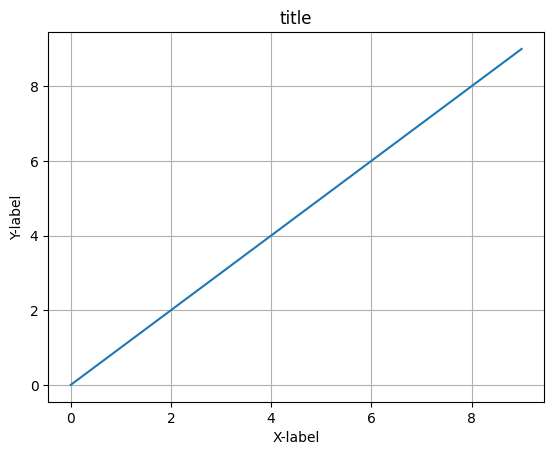
\includegraphics[width=0.6\linewidth]{image/tmp1.png}
  \caption{キャプション}
  \label{fig:fig1}
\end{figure}
% 画像2
\begin{figure}[H]
  \centering
  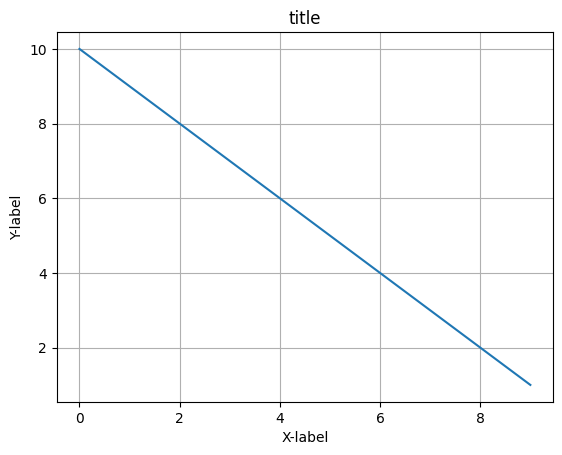
\includegraphics[width=0.6\linewidth]{image/tmp2.png}
  \caption{キャプション}
  \label{fig:fig2}
\end{figure}

\section{参考文献}

原稿の中で他の文献を引用する場合は，論文の最後に参考文献のリストを付けて
参照する必要がある．
\TeX には，参考文献のリストを作成するために用いる環境と文献の引用に用い
るコマンドが用意されており，参考文献のリストを作成するには
「thebibliography」環境を用いて次のように記述する． 
\begin{verbatim}
\begin{thebibliography}{9}
\bibitem{Okumura} 奥村晴彦「\LaTeXe 美文書作成入門」（技術評論社）
\bibitem{Yoshinaga} 吉永徹美「独習\LaTeXe 」（翔泳社）
\bibitem{Shimizu} 清水美樹「はじめての\LaTeX」（工学社）
\end{thebibliography}
\end{verbatim}
この場合，次のように出力される．
\begin{thebibliography}{9} %この位置に文献表を作成
\bibitem{Okumura} 奥村晴彦・黒木裕介「\LaTeXe 美文書作成入門（改訂第7版）」（技術評論社）
\bibitem{Yoshinaga} 吉永徹美「独習\LaTeXe 」（翔泳社）
\bibitem{Shimizu} 清水美樹「はじめての\LaTeX 」（工学社）
\end{thebibliography}

「thebibliography」環境の中で\verb+「\bibitem{ラベル名}+として文献のリス
トを記入する．
参考文献の番号付けのスタイルは，ドキュメントクラスに依存し，「jarticle」
クラスの場合，[1], [2] のように番号付けされる．
\verb+「\begin{thebibliography}{9}」+の「{9}」の部分では，番号付けで用い
る幅を指定する\footnote{この場合，「9」の幅の分だけ番号付けのスペースが確保される．文
献のリストが増えて 2 桁になる場合は，「9」を「99」に変更する．
%\verb+「\begin{thebibliography}{99}」+のように指定する．
}．

番号付けで自分で好きな番号を付けるためには，
\verb+\bibitem[番号]{ラベル名}+」とオプションで指定する．
このとき，番号付けで用いる幅に注意する必要がある．

\end{document}

